\section{ Topics covered}
\begin{itemize}
\item Risk management
\item Managing people
\item Teamwork
\end{itemize}

\section{ Software project management}
\begin{itemize}
\item Concerned with activities involved in ensuring that software is delivered on time and on schedule and in accordance with the requirements of the organisations developing and procuring the software.
\item Project management is needed because software development is always subject to budget and schedule constraints that are set by the organisation developing the software.
\end{itemize}

\subsection{ Success criteria}
\begin{itemize}
\item Deliver the software to the customer at the agreed time.
\item Keep overall costs within budget.
\item Deliver software that meets the customer’s expectations.
\item Maintain a happy and well-functioning development team.
\end{itemize}

\subsection{ Software management distinctions}
\begin{itemize}
\item \textbf{The product is intangible}.
\newline $-$Software cannot be seen or touched. Software project managers cannot see progress by simply looking at the artefact that is being constructed.
\item \textbf{Many software projects are 'one-off' projects}.
\newline $-$ Large software projects are usually different in some ways from previous projects. Even managers who have lots of previous experience may find it difficult to anticipate problems.
\item \textbf{Software processes are variable and organization specific}.
\newline $-$ We still cannot reliably predict when a particular software process is likely to lead to development problems.
\end{itemize}

\subsection{ Management activities}
\begin{enumerate}
\item \textbf{Project planning}
\newline $-$Project managers are responsible for planning. estimating and scheduling project development and assigning people to tasks.
\item \textbf{Reporting}
\newline $-$Project managers are usually responsible for reporting on the progress of a project to customers and to the managers of the company developing the software.
\item \textbf{Risk management}
\newline $-$Project managers assess the risks that may affect a project, monitor these risks and take action when problems arise.
\item \textbf{People management}
\newline $-$ Project managers have to choose people for their team and establish ways of working that leads to effective team performance
\item \textbf{Proposal writing}
\newline $-$ The first stage in a software project may involve writing a proposal to win a contract to carry out an item of work. The proposal describes the objectives of the project and how it will be carried out.
\end{enumerate}

\section{ Risk management}
Risk management is concerned with identifying risks and drawing up plans to minimise their effect on a project.
A risk is a probability that some adverse circumstance will occur

\begin{itemize}
  \item Project risks affect schedule or resources;
  \item Product risks affect the quality or performance of the software being developed;
  \item Business risks affect the organisation developing or procuring the software.

\end{itemize}

\newpage
\subsection{ Examples of common project, product, and business risks}

\begin{table}[h!]
\centering
\begin{tabular}{ |p{2cm}|p{2cm}|p{8cm}|  }
\hline
Risk & Affects & Description\\
\hline
\hline
Staff Turnover & Project & Experienced staff will leave the project before it is finished.\\
\hline
Management change & Project & There will be a change of organizational management with different priorities.\\
\hline
Hardware unavailability & Project & Hardware that is essential for the project will not be delivered on schedule.\\
\hline
Requirements change & Project \& Product & There will be a larger number of changes to the requirements than anticipated.\\
\hline
Specification delays & Project \& Product & Specifications of essential interfaces are not available on schedule.\\
\hline
Size underestimate & Project \& Product & The size of the system has been underestimated.\\
\hline
CASE tool underperformance & Product & CASE tools, which support the project, do not perform as anticipated.\\
\hline
Technology change & Business & The underlying technology on which the system is built is superseded by new technology.\\
\hline
Product competition & Business & A competitive product is marketed before the system is completed.\\
\hline
\end{tabular}

\label{table:T5_1}
\end{table}


\section{ The risk management process}
\begin{itemize}

\item Risk identification

  \item Identify project, product and business risks; \item Risk analysis
  \item Assess the likelihood and consequences of these risks; \item Risk planning
  \item Draw up plans to avoid or minimise the effects of the risk; \item Risk monitoring
  \item Monitor the risks throughout the project;

\end{itemize}

\section{ The risk management process}
\begin{figure}[h!]
    \centering
    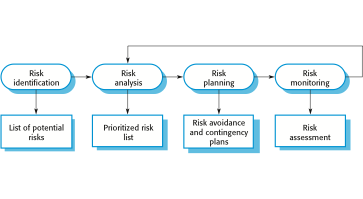
\includegraphics[width = 0.8\textwidth]{./figures/L5_1.png}
    \caption{}
    \label{fig:L5_1}
\end{figure}


\section{ Risk identification}
\begin{itemize}

\item May be a team activities or based on the individual project manager’s experience.

\item A checklist of common risks may be used to identify risks in a project

  \item Technology risks.   \item People risks.   \item Organisational risks.   \item Requirements risks.   \item Estimation risks.

\end{itemize}
\newpage
\section{ Examples of different risk types}
\begin{table}[h!]
\centering
\begin{tabular}{ |p{3cm}|p{8cm}|  }
\hline
Risk type & Possible risks \\
\hline
\hline
Technology & The database used in the system cannot process as many transactions per second as expected. (1)
Reusable software components contain defects that mean they cannot be reused as planned. (2)\\
\hline
People & It is impossible to recruit staff with the skills required. (3) Key staff are ill and unavailable at critical times. (4) Required training for staff is not available. (5)\\
\hline
Organizational & The organization is restructured so that different management are responsible for the project. (6)
Organizational financial problems force reductions in the project budget. (7)\\
\hline
Tools & The code generated by software code generation tools is inefficient. (8) Software tools cannot work together in an integrated way. (9)\\
\hline
Requirements & Changes to requirements that require major design rework are proposed. (10) Customers fail to understand the impact of requirements changes. (11)\\
\hline
Estimation & The time required to develop the software is underestimated. (12) The rate of defect repair is underestimated. (13)
The size of the software is underestimated. (14)\\

\hline
\end{tabular}

\label{table:T5_2}
\end{table}

\section{ Risk analysis}
\begin{itemize}

\item Assess probability and seriousness of each risk.

\item Probability may be very low, low, moderate, high or very high.

\item Risk consequences might be catastrophic, serious, tolerable or insignificant.


\end{itemize}
\newpage
\section{ Risk types and examples}
\begin{table}[h!]
\centering
\begin{tabular}{ |p{7cm}|p{2cm}|p{2cm}|  }
\hline
Risk & Probability &  Effects\\
\hline
\hline
Organizational financial problems force reductions in the project budget (7). & Low & Catastrophic\\
\hline
It is impossible to recruit staff with the skills required for the project (3). & High & atastrophic\\
\hline
Key staff are ill at critical times in the project (4). & Moderate & Serious\\
\hline
Faults in reusable software components have to be repaired before these components are reused. (2). & Moderate & Serious\\
\hline
Changes to requirements that require major design rework are proposed (10). & Moderate & Serious\\
\hline
The	organization	is	restructured	so	that	different management are responsible for the project (6). & High & Serious\\
\hline
The database used in the system cannot process as many transactions per second as expected (1). & Moderate & Serious\\
\hline
The	time	required	to	develop	the	software	is underestimated (12). & High & Serious\\
\hline
Software tools cannot be integrated (9). & High & Tolerable\\
\hline
Customers fail to understand the impact of requirements changes (11). & Moderate & Tolerable\\
\hline
Required training for staff is not available (5). & Moderate & Tolerable\\
\hline
The rate of defect repair is underestimated (13). & Moderate & Tolerable\\
\hline
The size of the software is underestimated (14). & High & Tolerable\\
\hline
Code generated by code generation tools is inefficient (8). & Moderate & Insignificant\\
\hline

\end{tabular}

\label{table:T5_2}
\end{table}


\section{ Risk planning}
\begin{itemize}

\item Consider each risk and develop a strategy to manage that risk.

\item Avoidance strategies

  \item The probability that the risk will arise is reduced; \item Minimisation strategies
  \item The impact of the risk on the project or product will be reduced; \item Contingency plans
  \item If the risk arises, contingency plans are plans to deal with that risk;
\end{itemize}

\section{Risk monitoring}
\begin{itemize}

\item Assess each identified risks regularly to decide whether or not it is becoming less or more probable.

\item Also assess whether the effects of the risk have changed.

\item Each key risk should be discussed at management progress meetings.

\end{itemize}

\section{ Key points}
\begin{itemize}

\item Good project management is essential if software engineering projects are to be developed on schedule and within budget.

\item Software management is distinct from other engineering management. Software is intangible. Projects may be novel or innovative with no body of experience to guide their management. Software processes are not as mature as traditional engineering processes.

\item Risk management is now recognized as one of the most important project management tasks.

\item Risk management involves identifying and assessing project risks to establish the probability that they will occur and the consequences for the project if that risk does arise. You should make plans to avoid, manage or deal with likely risks if or when they arise.

\end{itemize}

\newpage
\section{ Strategies to help manage risk}
\begin{table}[h!]
\centering
\begin{tabular}{ |p{4cm}|p{8cm}|  }
\hline
Risk & Strategy\\
\hline
\hline
Organizational financial problems & Prepare a briefing document for senior management showing how the project is making a very important contribution to the goals of the business and presenting reasons why cuts to the project budget would not be cost-effective.\\
\hline
Recruitment problems & Alert customer to potential difficulties and the possibility of delays; investigate buying-in components.\\
\hline
Staff illness & Reorganize team so that there is more overlap of work and people therefore understand each other’s jobs.\\
\hline
Defective components & Replace potentially defective components with bought-in components of known reliability.\\
\hline
Requirements changes & Derive traceability information to assess requirements change impact; maximize information hiding in the design.\\
\hline
Organizational restructuring & Prepare a briefing document for senior management showing how the project is making a very important contribution to the goals of the business.\\
\hline
Database performance & Investigate the possibility of buying a higher-performance database.\\
\hline
Underestimated development time & Investigate buying-in components; investigate use of a program generator.\\
\hline

\end{tabular}

\label{table:T5_3}
\end{table}

\newpage
\section{ Risk indicators}
\begin{table}[h!]
\centering
\begin{tabular}{ |p{4cm}|p{8cm}|  }
\hline
Risk type & Potential indicators\\
\hline
\hline
Technology & Late delivery of hardware or support software; many reported technology problems.\\
\hline
People & Poor staff morale; poor relationships amongst team members; high staff turnover.\\
\hline
Organizational & Organizational gossip; lack of action by senior management.\\
\hline
Tools & Reluctance by team members to use tools; complaints about CASE tools; demands for higher-powered workstations.\\
\hline
Requirements & Many requirements change requests; customer complaints.\\
\hline
Estimation & Failure to meet agreed schedule; failure to clear reported defects.\\
\hline

\end{tabular}

\label{table:T5_4}
\end{table}


\section{ Managing people}
\begin{itemize}

\item People are an organisation’s most important assets.

\item The tasks of a manager are essentially people-oriented. Unless there is some understanding of people, management will be unsuccessful.

\item Poor people management is an important contributor to project failure.
\end{itemize} \section{ People management factors}
\begin{itemize}

\item Consistency

  \item Team members should all be treated in a comparable way without favourites or discrimination.

\item Respect

  \item Different team members have different skills and these differences should be respected.

\item Inclusion

  \item Involve all team members and make sure that people’s views are considered.

\item Honesty

  \item You should always be honest about what is going well and what is going badly in a project.
\end{itemize} \section{ Motivating people}
\begin{itemize}

\item An important role of a manager is to motivate the people working on a project.

\item Motivation means organizing the work and the working environment to encourage people to work effectively.

  \item If people are not motivated, they will not be interested in the work they are doing. They will work slowly, be more likely to make mistakes and will not contribute to the broader goals of the team or the organization.

\item Motivation is a complex issue but it appears that their are different types of motivation based on:

  \item Basic needs (e.g. food, sleep, etc.);   \item Personal needs (e.g. respect, self-esteem);
  \item Social needs (e.g. to be accepted as part of a group).

\end{itemize}
\section{ Human needs hierarchy}
\begin{figure}[h!]
    \centering
    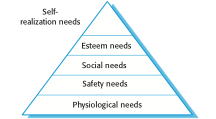
\includegraphics[width = 0.8\textwidth]{./figures/L5_2.png}
    \caption{}
    \label{fig:L5_2}
\end{figure}


\section{ Need satisfaction}
\begin{itemize}

\item In software development groups, basic physiological and safety needs are not an issue.

\item Social

  \item Provide communal facilities;
  \item Allow informal communications e.g. via social networking \item Esteem
  \item Recognition of achievements;   \item Appropriate rewards.
\item Self-realization

  \item Training - people want to learn more;   \item Assigning Responsibility.


\end{itemize}
\section{ Individual motivation}


Alice is a software project manager working in a company that develops alarm systems. This company wishes to enter the growing market of assistive technology to help elderly and disabled people live independently. Alice has been asked to lead a team of 6 developers than can develop new products based around the company’s alarm technology.


Alice’s assistive technology project starts well. Good working relationships develop within the team and creative new ideas are developed. The team decides to develop a peer-to-peer messaging system using digital televisions linked to the alarm network for communications. However, some months into the project, Alice notices that Dorothy, a hardware design expert, starts coming into work late, the quality of her work deteriorates and, increasingly, that she does not appear to be communicating with other members of the team.
Alice talks about the problem informally with other team members to try to find out if Dorothy’s personal circumstances have changed, and if this might be affecting her work. They don’t know of anything, so Alice decides to talk with Dorothy to try to understand the problem.

After some initial denials that there is a problem, Dorothy admits that she has lost interest in the job. She expected that she would be able to develop and use her hardware interfacing skills. However, because of the product direction that has been chosen, she has little opportunity for this. Basically, she is working as a C programmer with other team members.


Although she admits that the work is challenging, she is concerned that she is not developing her interfacing skills. She is worried that finding a job that involves hardware interfacing will be difficult after this project. Because she does not want to upset the team by revealing that she is thinking about the next project, she has decided that it is best to minimize conversation with them.

\subsection{Solution to Dorithy’s Problem}
\begin{itemize}
\item Give her autonomy in designing

\item Give her training on software engineering

\item She will be motivated in the new work


\end{itemize} \section{ Different Motivations for Different Personality types}
\begin{itemize}

\item The needs hierarchy is almost certainly an over-simplification of motivation in practice.

\item Motivation should also take into account different personality types: (Different People are Motivated in Different ways)

  \item Task-oriented;   \item Self-oriented;   \item Interaction-oriented.


\end{itemize} \section{ Different Motivations for Different Personality types}
\begin{itemize}
\item Task-oriented.

  \item The motivation for doing the work is the work itself;   \item Acts as individuals
\item Self-oriented.

  \item The work is a means to an end which is the achievement of individual goals - e.g. to get rich, to play tennis, to travel etc.;
  \item Acts as individuals \item Interaction-oriented
  \item The principal motivation is the presence and actions of co-workers. People go to work because they like to go to work.
  \item Mostly female workers

\end{itemize}
\section{ Motivation balance}
\begin{itemize}


\item Individual motivations are made up of elements of each class.

  \item One personality type must be dominant

\item The personality can change depending on personal circumstances and external events.

\item However, people are not just motivated by personal factors but also by being part of a group and culture.

\item People go to work because they are motivated by the people that they work with.

\end{itemize}
\section{ Teamwork}

\begin{itemize}

\item Most software engineering is a group activity

  \item The development schedule for most non-trivial software projects is such that they cannot be completed by one person working alone.

\item A good group is cohesive and has a team spirit. The people involved are motivated by the success of the group as well as by their own personal goals.

\item Group interaction is a key determinant of group performance.

\item Flexibility in group composition is limited

  \item Managers must do the best they can with available people.

\end{itemize} \section{ Group cohesiveness}
\begin{itemize}

\item In a cohesive group, members consider the group to be more important than any individual in it.

\item The advantages of a cohesive group are:

  \item Group quality standards can be developed by the group members.
  \item Team members learn from each other and get to know each other’s work; Inhibitions caused by ignorance are reduced.
  \item Knowledge is shared. Continuity can be maintained if a group member leaves.
  \item Refactoring and continual improvement is encouraged. Group members work collectively to deliver high quality results and fix problems, irrespective of the individuals who originally created the design or program.
\end{itemize}
 \section{ Team spirit}


Alice, an experienced project manager, understands the importance of creating a cohesive group. As they are developing a new product, she takes the opportunity of involving all group members in the product specification and design by getting them to discuss possible technology with elderly members of their families. She also encourages them to bring these family members to meet other members of the development group.


Alice also arranges monthly lunches for everyone in the group. These lunches are an opportunity for all team members to meet informally, talk around issues of concern, and get to know each other. At the lunch, Alice tells the group what she knows about organizational news, policies, strategies, and so forth. Each team member then briefly summarizes what they have been doing and the group discusses a general topic, such as new product ideas from elderly relatives.


Every few months, Alice organizes an ‘away day’ for the group where the team spends two days on ‘technology updating’. Each team member prepares an update on a relevant technology and presents it to the group. This is an off-site meeting in a good hotel and plenty of time is scheduled for discussion and social interaction.
\section{ The effectiveness of a team}
\begin{itemize}

\item The people in the group

  \item You need a mix of people in a project group as software development involves diverse activities such as negotiating with clients, programming, testing and documentation.

\item The group organization

  \item A group should be organized so that individuals can contribute to the best of their abilities and tasks can be completed as expected.

\item Technical and managerial communications

  \item Good communications between group members, and between the software engineering team and other project stakeholders, is essential.

\end{itemize}
\section{ Selecting group members}
\begin{itemize}

\item A manager or team leader’s job is to create a cohesive group and organize their group so that they can work together effectively.

\item This involves creating a group with the right balance of technical skills and personalities, and organizing that group so that the members work together effectively.


\end{itemize}
\section{ Assembling a team}
\begin{itemize}

\item May not be possible to appoint the ideal people to work on a project

  \item Project budget may not allow for the use of highly-paid staff;   \item Staff with the appropriate experience may not be available;
  \item An organisation may wish to develop employee skills on a software project.

\item Managers have to work within these constraints especially when there are shortages of trained staff.

\end{itemize} \section{ Group composition}
\begin{itemize}

\item Group composed of members who share the same motivation can be problematic

  \item Task-oriented - everyone wants to do their own thing;   \item Self-oriented - everyone wants to be the boss;   \item Interaction-oriented - too much chatting, not enough work.
\item An effective group has a balance of all types.

\item This can be difficult to achieve software engineers are often task-oriented.

\item Interaction-oriented people are very important as they can detect and defuse tensions that arise.


\end{itemize}
\section{ Group composition}


In creating a group for assistive technology development, Alice is aware of the importance of selecting members with complementary personalities. When interviewing potential group members, she tried to assess whether they were task-oriented, self-oriented, or interaction-oriented. She felt that she was primarily a self-oriented type because she considered the project to be a way of getting noticed by senior management and possibly promoted. She therefore looked for one or perhaps two interaction-oriented personalities, with task-oriented individuals to complete the team. The final assessment that she arrived at was:


Alice-self-oriented Brian—task-oriented Bob-task-oriented Carol-interaction-oriented Dorothy-self-oriented Ed-interaction-oriented Fred-task-oriented

\section{Group organization}
\begin{itemize}

\item The way that a group is organized affects the decisions that are made by that group, the ways that information is exchanged and the interactions between the development group and external project stakeholders.

\item Key questions include:
\newline $-$Should the project manager be the technical leader of the group?
\newline $-$Who will be involved in making critical technical decisions, and how will these be made?
\newline $-$How will interactions with external stakeholders and senior company management be handled?
\newline $-$How can groups integrate people who are not co-located? • How can knowledge be shared across the group?

\item Small software engineering groups are usually organised informally without a rigid structure.

\item For large projects, there may be a hierarchical structure where different groups are responsible for different sub-projects.

\item Agile development is always based around an informal group on the principle that formal structure inhibits information exchange

\end{itemize}
\section{ Informal groups}
\begin{itemize}

\item The group acts as a whole and comes to a consensus on decisions affecting the system.

\item The group leader serves as the external interface of the group but does not allocate specific work items.

\item Rather, work is discussed by the group as a whole and tasks are allocated according to ability and experience.

\item This approach is successful for groups where all members are experienced and competent.

\end{itemize}
\section{ Group communications}
\begin{itemize}

\item Good communications are essential for effective group working.

\item Information must be exchanged on the status of work, design decisions and changes to previous decisions.

\item Good communications also strengthens group cohesion as it promotes understanding.


\end{itemize}
\section{ Group communications}
\begin{itemize}

\item Group size

  \item The larger the group, the harder it is for people to communicate with other group members.

\item Group structure

  \item Communication is better in informally structured groups than in hierarchically structured groups.

\item Group composition

  \item Communication is better when there are different personality types in a group and when groups are mixed rather than single sex.

\item The physical work environment

  \item Good workplace organisation can help encourage communications.

\end{itemize}
\section{ Key points}
\begin{itemize}

\item People are motivated by interaction with other people, the recognition of management and their peers, and by being given opportunities for personal development.

\item Software development groups should be fairly small and cohesive. The key factors that influence the effectiveness of a group are the people in that group, the way that it is organized and the communication between group members.

\item Communications within a group are influenced by factors such as the status of group members, the size of the group, the gender composition of the group, personalities and available communication channels.
\end{itemize}
